% fig_87L_hif_response.tex
% Bar chart: 87L I_fund and f_int for HIF line scenarios (alpha=0.05 ag)
% across 4 topologies, showing consistent detection above threshold
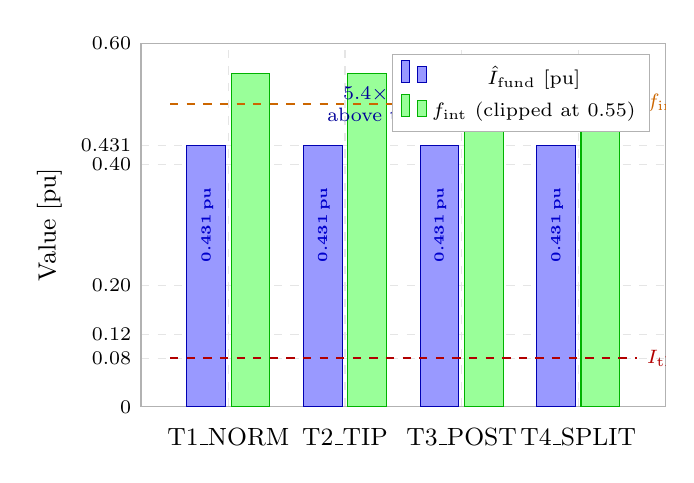
\begin{tikzpicture}
\begin{axis}[
  name            = hifax,
  ybar,
  bar width       = 14pt,
  width           = 0.68\textwidth,
  height          = 6.2cm,
  enlarge x limits= 0.25,
  ylabel          = {Value [pu]},
  ylabel style    = {font=\small},
  ymin            = 0,
  ymax            = 0.60,
  ytick           = {0, 0.08, 0.12, 0.20, 0.40, 0.431, 0.60},
  yticklabels     = {0, 0.08, 0.12, 0.20, 0.40, 0.431, 0.60},
  yticklabel style= {font=\scriptsize},
  xtick           = {1,2,3,4},
  xticklabels     = {T1\_NORM, T2\_TIP, T3\_POST, T4\_SPLIT},
  xticklabel style= {font=\small},
  legend style    = {at={(0.97,0.97)}, anchor=north east,
                     font=\scriptsize, draw=gray!60},
  legend columns  = 1,
  grid            = major,
  grid style      = {gray!20, dashed},
  tick style      = {draw=none},
  axis line style = {gray!60},
]

% I_fund bars (blue) — all 0.431 pu
\addplot[fill=blue!40, draw=blue!70!black]
  coordinates {(1,0.431) (2,0.431) (3,0.431) (4,0.431)};
\addlegendentry{$\hat{I}_{\rm fund}$ [pu]}

% f_int bars (green) — all 1.0 (clipped to 0.55 for display)
\addplot[fill=green!40, draw=green!70!black]
  coordinates {(1,0.55) (2,0.55) (3,0.55) (4,0.55)};
\addlegendentry{$f_{\rm int}$ (clipped at 0.55)}

% ---- Threshold lines -------------------------------------------------------
\draw[red!70!black, thick, dashed]
  (axis cs:0.5, 0.08) -- (axis cs:4.5, 0.08)
  node[right, font=\scriptsize, red!70!black] {$I_{\rm thresh}$=0.08};

\draw[orange!80!black, thick, dashed]
  (axis cs:0.5, 0.50) -- (axis cs:4.5, 0.50)
  node[right, font=\scriptsize, orange!80!black] {$f_{\rm int,trip}$=0.50};

% ---- Value annotations -----------------------------------------------------
\node[font=\tiny\bfseries, blue!80!black, rotate=90]
  at (axis cs:0.82, 0.30) {0.431\,pu};
\node[font=\tiny\bfseries, blue!80!black, rotate=90]
  at (axis cs:1.82, 0.30) {0.431\,pu};
\node[font=\tiny\bfseries, blue!80!black, rotate=90]
  at (axis cs:2.82, 0.30) {0.431\,pu};
\node[font=\tiny\bfseries, blue!80!black, rotate=90]
  at (axis cs:3.82, 0.30) {0.431\,pu};

% ---- Margin annotation -----------------------------------------------------
\node[font=\scriptsize, blue!60!black, align=center]
  at (axis cs:2.5, 0.50)
  {5.4$\times$ margin\\above threshold};

\end{axis}
\end{tikzpicture}
